Using the datasets from University of California Irvine Machine Learning Repository~\cite{uci_datasets}:

\begin{itemize}
\item Cardiac arrythmia dataset~\cite{dataset_cardiac_arythmia}, dataset with 452 instances and a big number of attributes - 279, representing attributes of people having cardiac arrythmia and their organs' states,
\item Handwritten numerals dataset~\cite{dataset_handwritten_numerals}, this dataset consists of features of handwritten numerals ($0$ - $9$) extracted from a collection of Dutch utility maps. 200 patterns per class (for a total of 2,000 patterns) with 64 attributes have been digitized in  binary images and represented in terms of few feature sets that are defined in referenced \emph{arff} file~\cite{dataset_handwritten_numerals},
\item Steel plates faults dataset~\cite{dataset_steel_plates_faults}, describing faults of steel plates like, e.g.: scratches, depth of the scratch, bumps or height of bump. This dataset totals to 1941 instances with 33 attributes each.
\end{itemize}

While using the implemented solution with aforementioned datasets, parameter $k = 30$ has been chosen to calculate the results.

%------------------------------------------
\subsection{Cardiac arrythmia dataset}
\label{subsec:cardiac}
In Figure~\ref{fig:graph_arrythmia_pearson} one can see cardiac arrythmia dataset visualization produced by implemented solution software.
Assortativity coefficient is stabilizing at around $0.31$ indicating assortative mixing.
Between $k$ 1 and 2 we can observe change in assortativity from disassortative to assortative.

Skewness of in-degrees is oscilating around level of $1.4 - 1.5$.
Its level indicates hubs phenomena present in this dataset.

\begin{figure}[h!]
  \centering
  \captionsetup{justification=centering}
    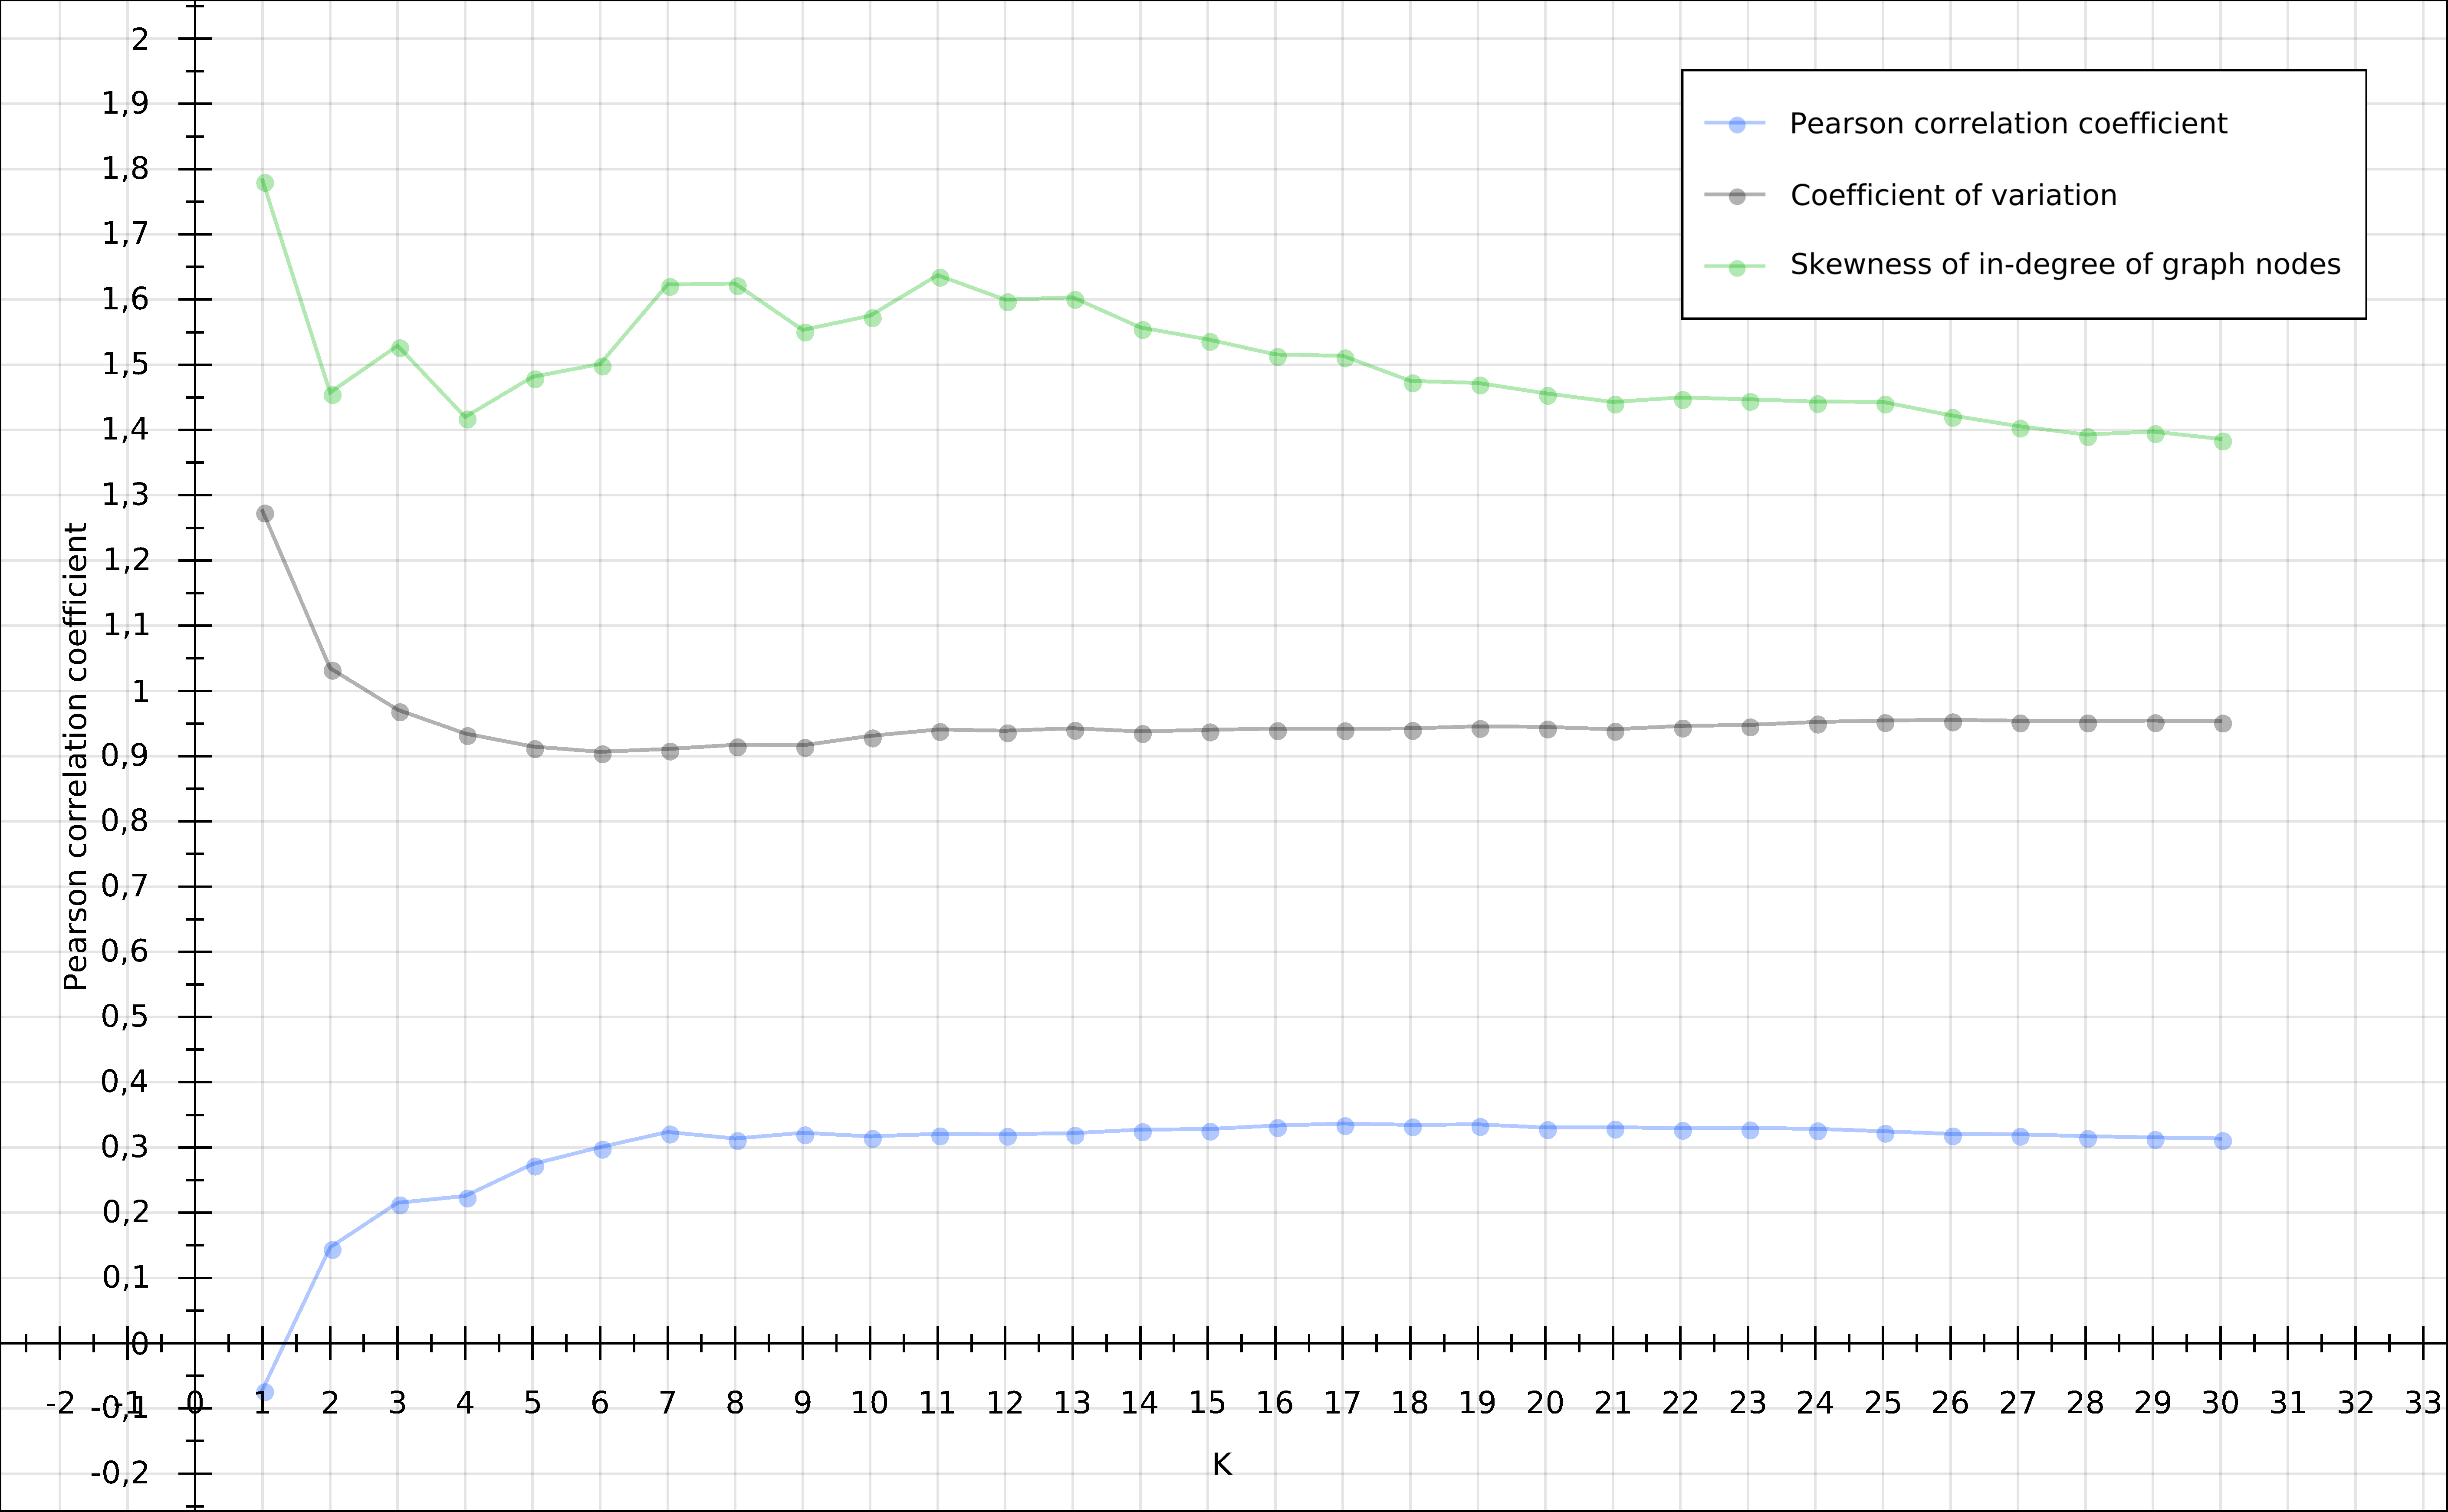
\includegraphics[width=0.95\textwidth]{images/arrythmia_pearson.png}
  \caption{Graph of Pearson correlation coefficient, its coefficient of variation and skewness of in-degree of nodes against $k$ parameter for cardiac arrythmia dataset.}
  \label{fig:graph_arrythmia_pearson}
\end{figure}


%------------------------------------------
\subsection{Handwritten numerals dataset}
Handwritten numerals dataset, presented with visualization in Figure~\ref{fig:graph_mfeat_pearson}, exhibits lower level of stable assortativity index level, at around $0.27$.
In this dataset we can see smaller gap between Pearson correlation coefficient and both skewness and coefficient of variation.

Similarily to cardiac arrythmia dataset in Section~\ref{subsec:cardiac} we can observe a change of assortativity between $k$ 1 and 2 from disassortative to assortative.

Positive skewness of in-degrees proves presence of hubs in kNN graph to be built upon this dataset.

\begin{figure}[h!]
  \centering
  \captionsetup{justification=centering}
    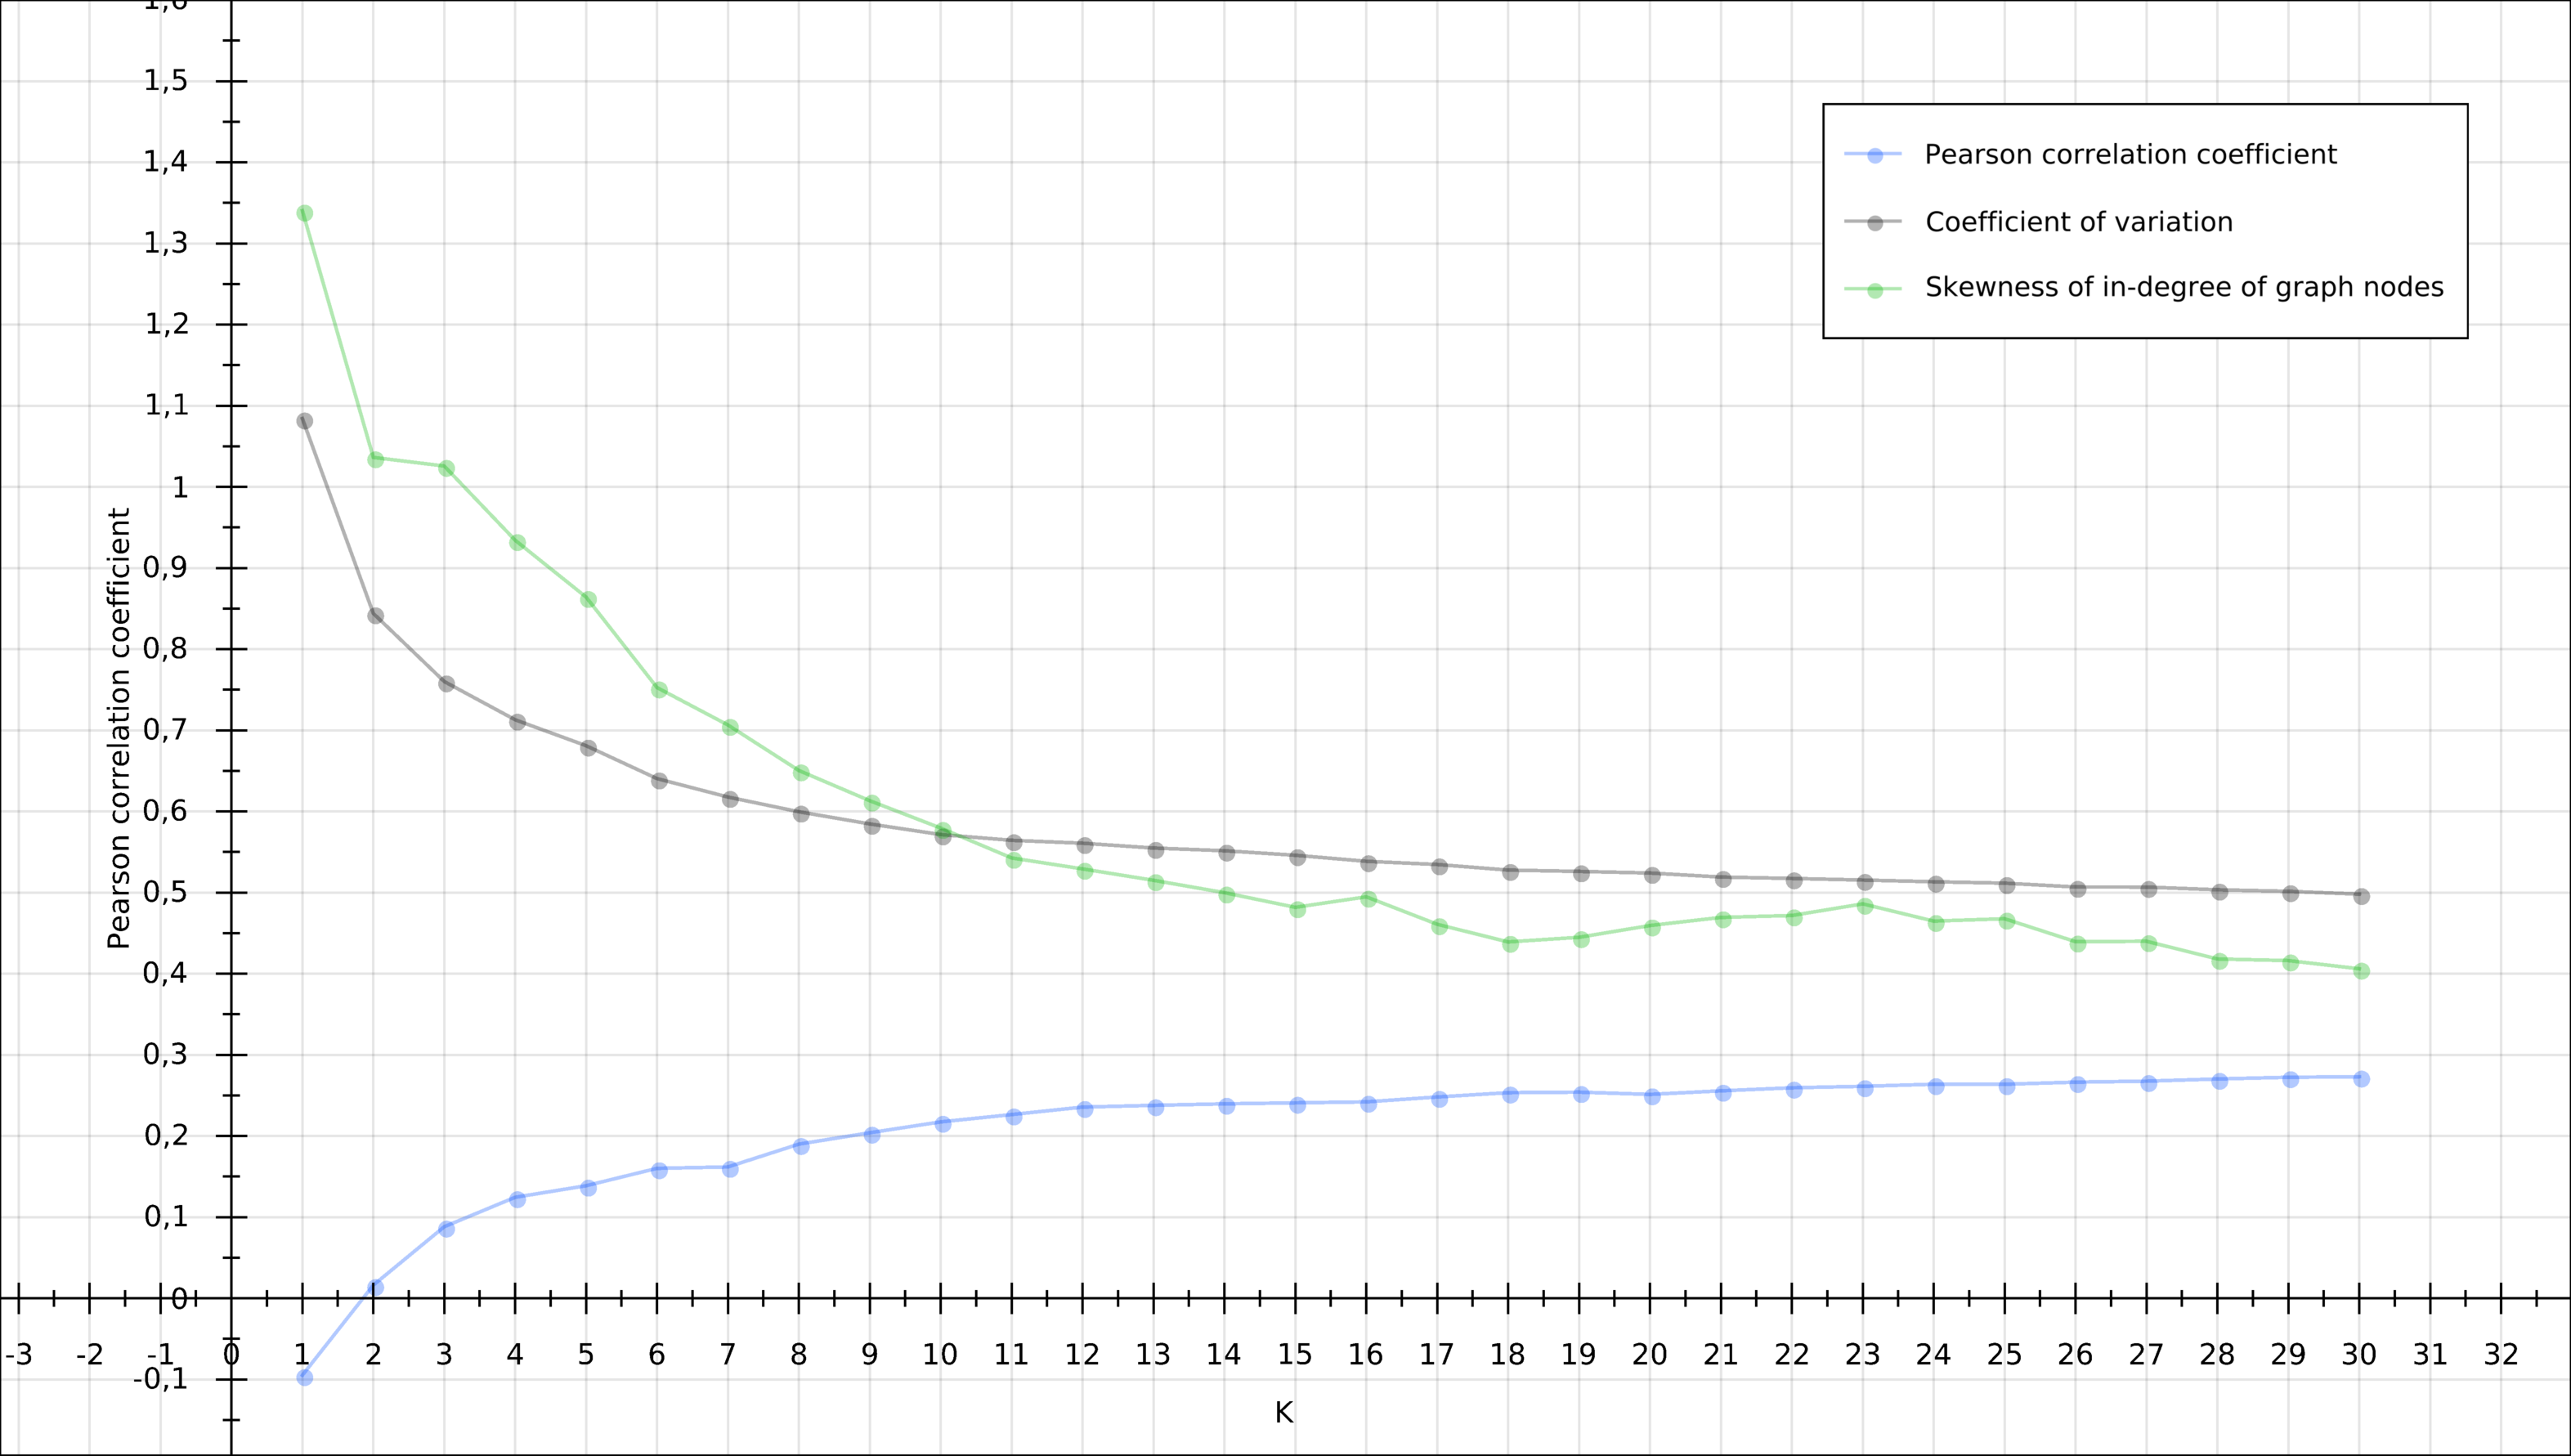
\includegraphics[width=0.95\textwidth]{images/mfeat_pearson.png}
  \caption{Graph of Pearson correlation coefficient, its coefficient of variation and skewness of in-degree of nodes against $k$ parameter for handwritten numerals dataset.}
  \label{fig:graph_mfeat_pearson}
\end{figure}


\clearpage
%------------------------------------------
\subsection{Steel plate faults dataset}
Steel plate faults dataset exhibits quite different parameters than 2 previous ones.
As one observe in Figure~\ref{fig:graph_faults_pearson}, its Pearson correlation coefficient of degrees between connected nodes stabilizes at around $0.31$ as in previous examples yet covariance of variation of nodes in-degrees descends below level of $0.3$ overlapping with assortativity index.

Skewness of nodes' in-degrees descends to negative values up until $-1.2$ for $k = 30$ indicating absence of hubness phenomena.

\begin{figure}[h!]
  \centering
  \captionsetup{justification=centering}
    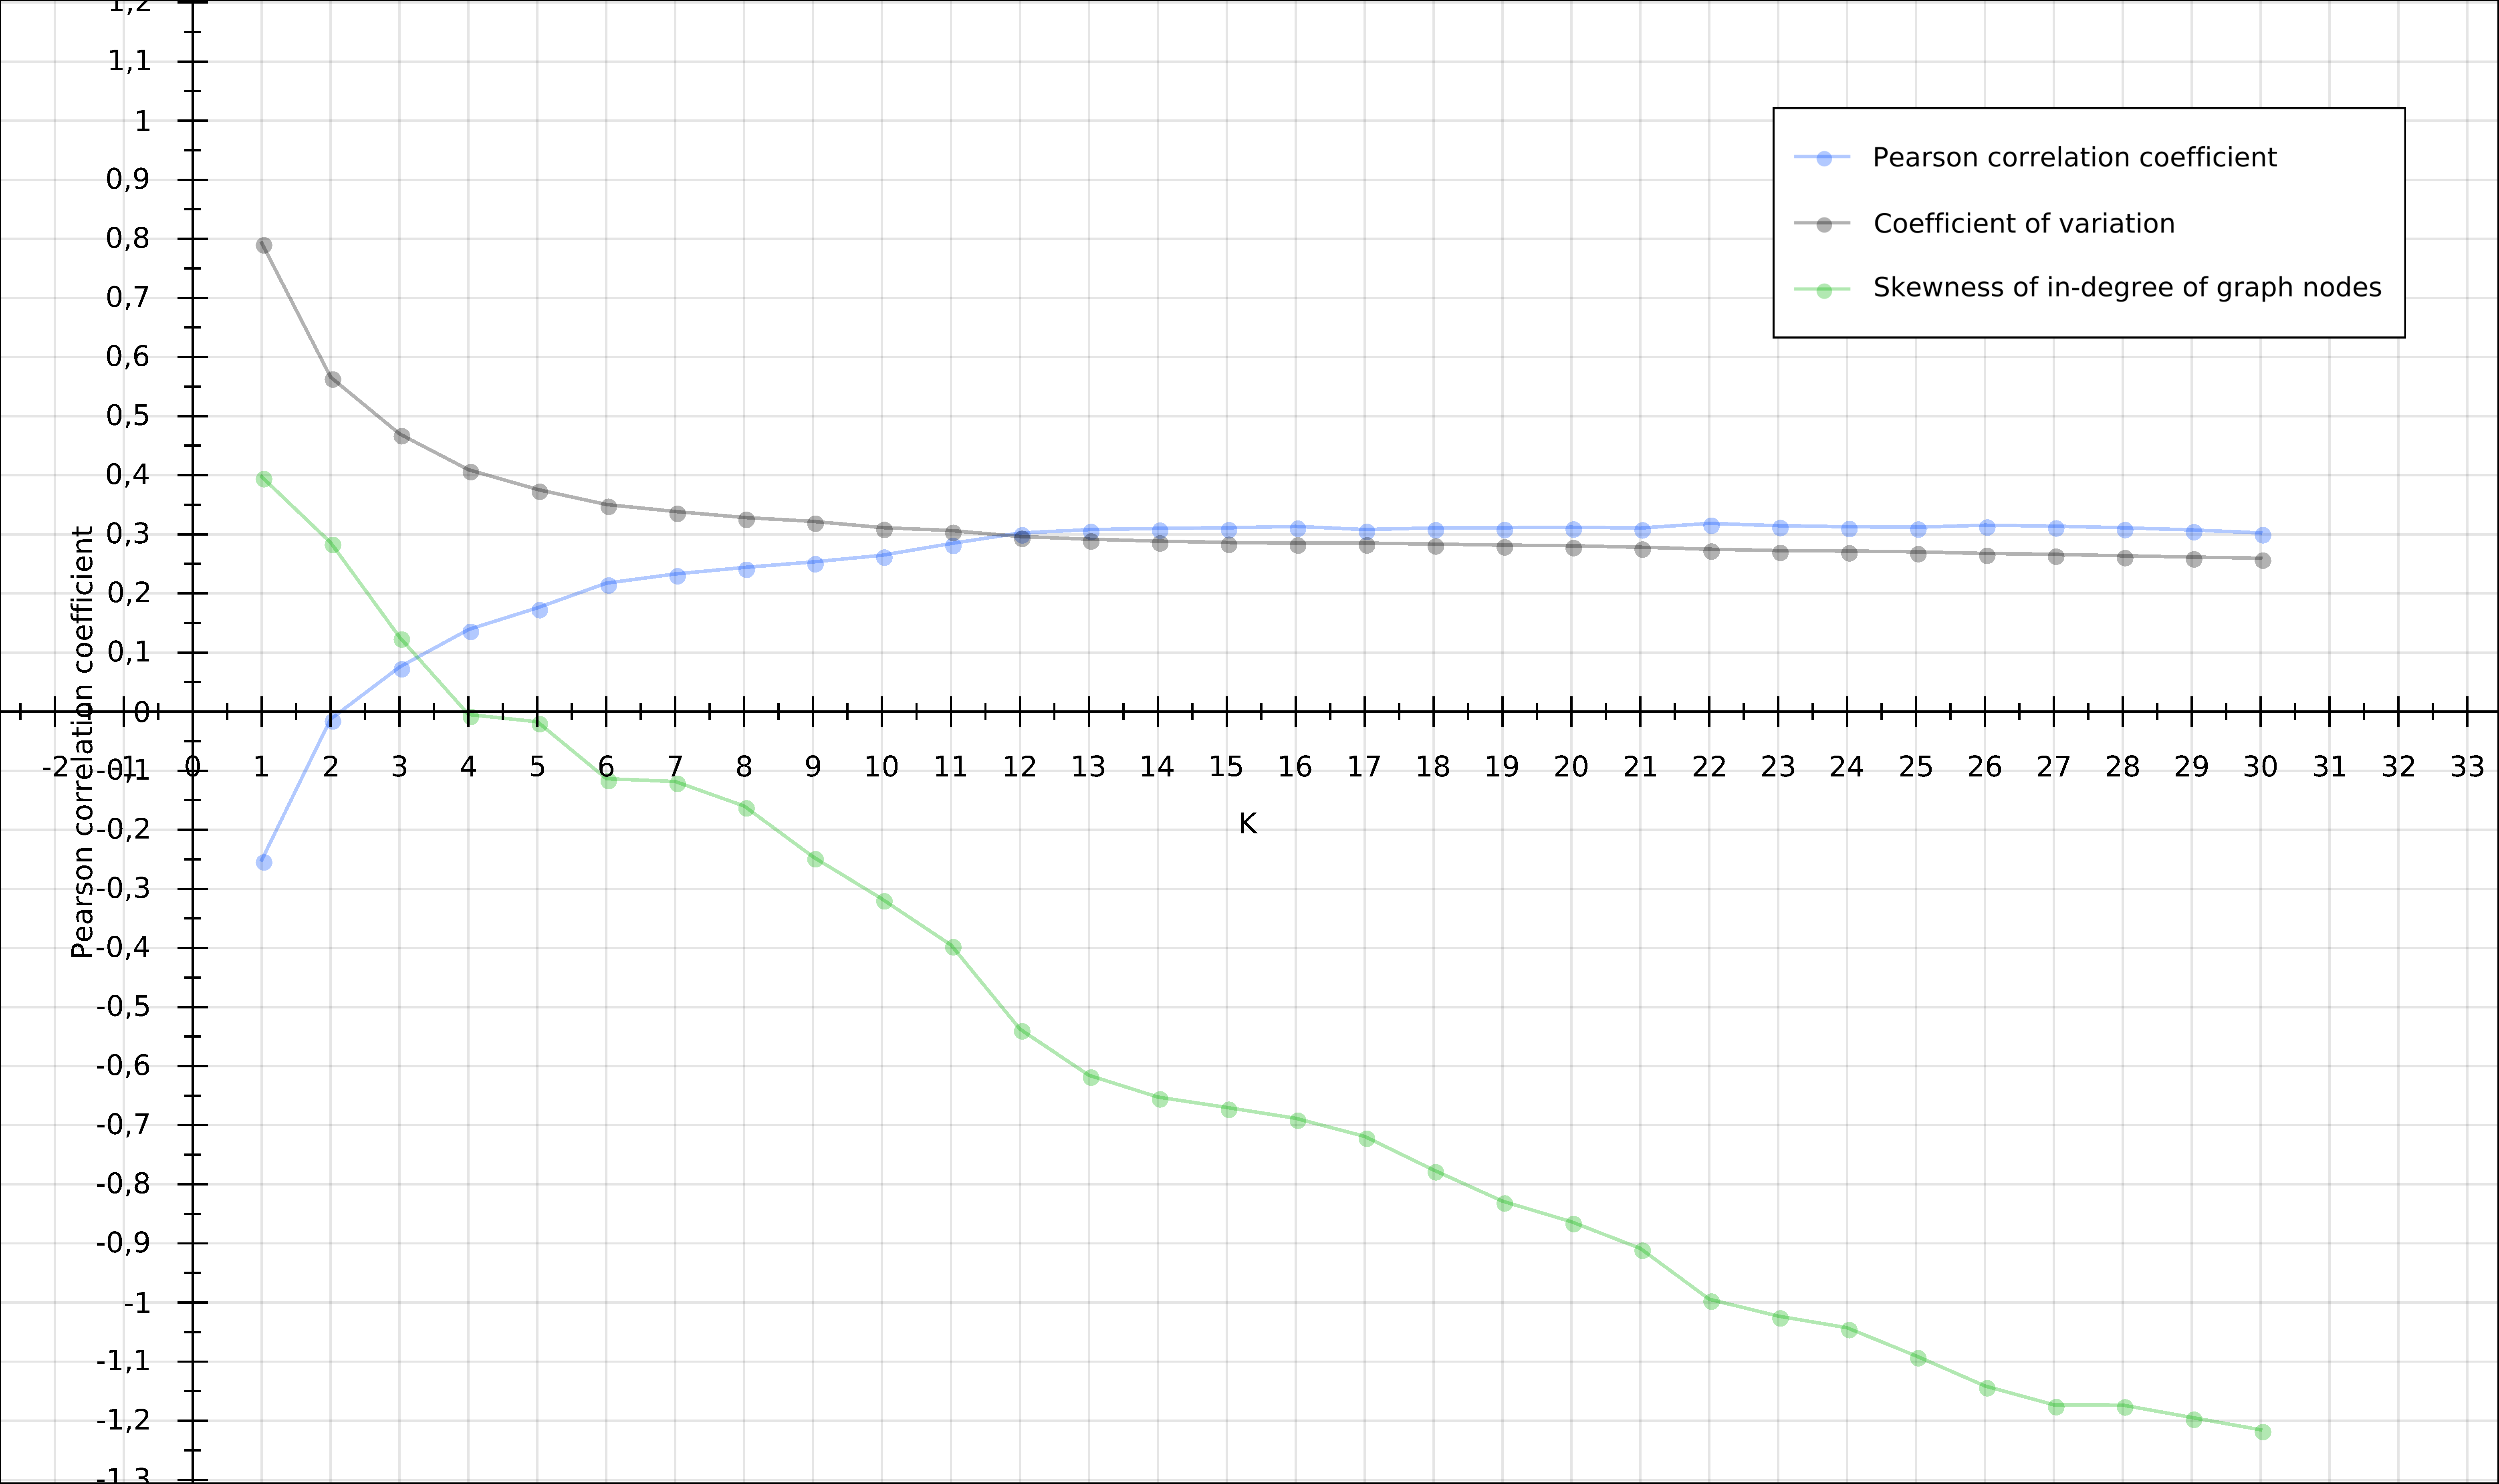
\includegraphics[width=0.95\textwidth]{images/faults_pearson.png}
  \caption{Graph of Pearson correlation coefficient, its coefficient of variation and skewness of in-degree of nodes against $k$ parameter for steel plates faults dataset.}
  \label{fig:graph_faults_pearson}
\end{figure}


In Figure~\ref{fig:graph_faults_nodes} one can observe tendency of nodes to connect to similar ones.
Red nodes constitute upper 25 percentile of the sample (calculated by the sume of node's values).

\begin{figure}[h!]
  \centering
  \captionsetup{justification=centering}
    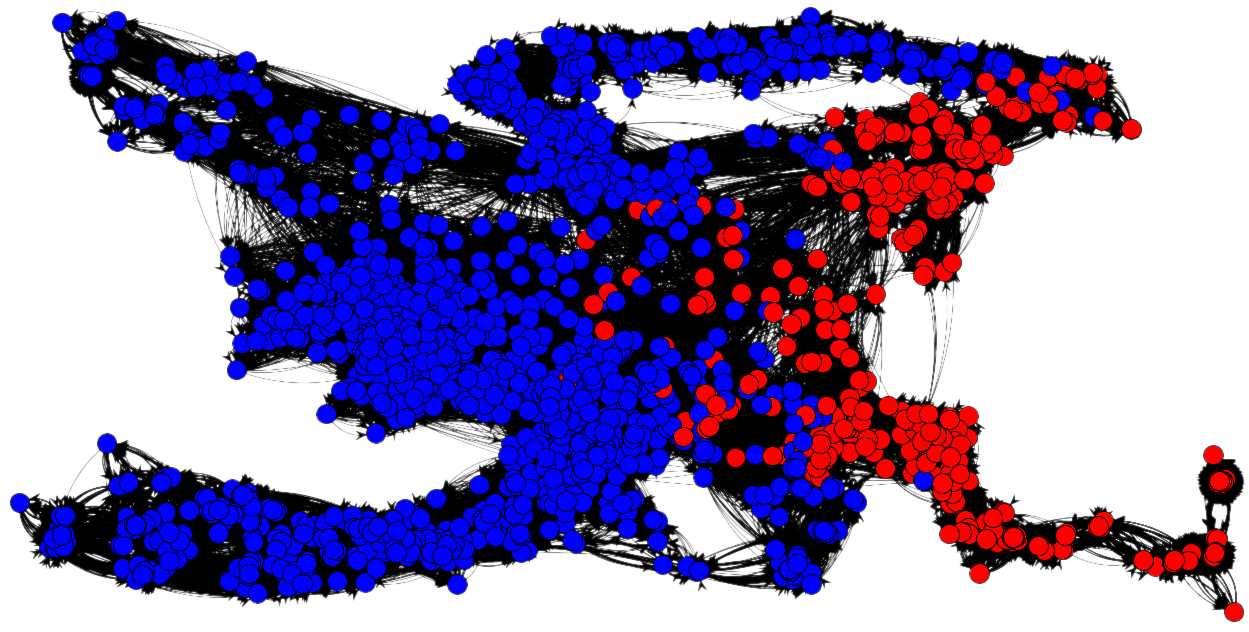
\includegraphics[width=0.95\textwidth]{images/faults_graph.png}
  \caption{K-NN graph representation of steel plates faults dataset with red nodes being the upper 25 perentile of dataset. This graph is showing medium positive assortativity coefficient of $0.30243338685364907$ which exhibits in nodes being connected to similar ones.}
  \label{fig:graph_faults_nodes}
\end{figure}

%------------------------------------------
\subsection{General conclusions}
General conclusion taken from aforementioned 3 datasets are as follows:
\begin{itemize}
\item k-NN graphs tend to be dissasortative or show no (dis)assortative mixing for small k ($k = 1$),
\item k-NN graphs tend to be assortative for large $k$,
\item assortativity for large $k$s occurs regardless of hubness phenomena ( e.g. both cardiac arrythmia dataset steel plates faults dataset positively assortative with and without hubs respectively) 
\end{itemize}


%------------------------------------------
\subsection{Analysis of results and follow-up work}
The main drawback of used method and solutions is that it has been performed on a very limited amount of datasets therefore it can be expanded in future work to minimize any deviations and/or noise in the datasets.
The follow-up work can also extend to investigate the hubness of networks in more detail.
Implemented solution can be improved to use whole processing power of the host machine by implementing better multithreading support.
